%\chapter{Funções exponenciais e logarítmicas}
 \chapter{Funções exponenciais}

\begin{obs}
 A função $f: \R \rightarrow \R$ dada por
\begin{equation*}
f(x) = a^x
\end{equation*}
 com $a>0$ e $a \neq 1$ é denominada função exponencial de base $a$ definida para todo $x$ real.
\end{obs}

 Observe que:
 \begin{itemize}
 \item Sempre temos que $f(0)=1$, ou seja, o gráfico de $a^x$ deve passar pelo ponto $(0,1)$;
 \item $a^x > 0$ para todo $x\in\R$;
 \item o maior domínio é o conjunto dos números reais;
 \item a imagem da função de domínio real é o conjunto dos números estritamente positivos $\R_{+}^*$.
  \item exigimos que a constante $a$ fosse positiva para garantir que a função estivesse definida para todo $x$ real (lembre-se que, por exemplo, $\sqrt{a}= a^{\frac{1}{2}}$ não está definida para $a$ negativo);
  \item excluímos $a=1$, pois $1^x=1$ para todo $x$ real, de modo que $f(x)= 1^x$ é uma função constante.
 \end{itemize}

 \begin{exem}\label{ex:exp-2}
  Considere a função $f: \R \rightarrow \R $ dada por,
\begin{equation*}
f(x) = 2^x \ , 
\end{equation*}
  
  Vamos determinar alguns pontos do gráfico da função $f$.

  \begin{table}[H]
  \centering
  \begin{tabular}{|c|c|} \hline
  \rowcolor{gray}
  $x$ & $y=2^x$ \\ \hline
  $-2$ & $\frac{1}{4}$ \\ \hline
  $-1$ & $\frac{1}{2}$ \\ \hline
  $0$ &  $1$ \\ \hline
  $1$ &  $2$ \\ \hline
  $2$ &  $4$ \\ \hline
  \end{tabular}
  \end{table}

  Marcando estes pontos no plano cartesiano e ligando obtemos o seguinte gráfico para esta função.

    \begin{center}
    \begin{tikzpicture}[scale=1]
    \tkzInit[xmin=-2.5, xmax=2.5, ymin=0,ymax=5]
        %\tkzDrawXY
        \tkzAxeXY[fill=black!5]
        
        \tkzFct[thick,red,samples=50,domain=-2.5:2.5]{2**x}
        \tkzDrawPoint[fill=red, size=3](0,1)
        \tkzDrawPoint[fill=red, size=3](1,2)
        \tkzDrawPoint[fill=red, size=3](2,4)
        \tkzDrawPoint[fill=red, size=3](-1,0.5)
        \tkzDrawPoint[fill=red, size=3](-2,0.25)

        %\draw[red, above right] (2,1) node{$f(x)$};
        %\draw[blue, above right] (1,2) node{$f^{-1}(x)$};
        %\tkzDefPointByFct[ref=A, with=a](-1)
        %\tkzDefPoint(0,4){A}
        %\tkzDefPoint(2,0){B}
        %\tkzPointShowCoord(A)
        %\tkzDrawPoint[fill=red, size=3](A)
        %\tkzDrawPoint[fill=red, size=3](B)
    \end{tikzpicture}
    \end{center}
    
  % \begin{figure}[H]
  % \centering
  %   \fbox{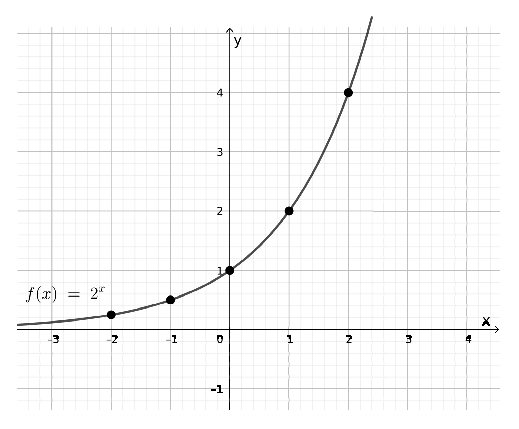
\includegraphics[width=7cm]{./cap_explog/figs/f(x)=2^x}}
  %   \caption{Gráficos da função $f(x)=2^x$}
  % \end{figure}

  Observe que neste caso a função é crescente, veremos que sempre que $a>1$ a função exponencial $f(x)=a^x$ será crescente e seu gráfico será parecido com este.

 \end{exem}


  \begin{exem}\label{ex:exp-1/2}
  Considere a função $f: \R \rightarrow \R$ dada por,
\begin{equation*}
f(x) = \left(\dfrac{1}{2}\right)^x \ , 
\end{equation*}
  vamos determinar alguns pontos do gráfico da função $f$.

  \begin{table}[H]
  \centering
  \begin{tabular}{|c|c|} \hline
  \rowcolor{gray}
  $x$ &  $y=(\frac{1}{2})^x$ \\ \hline
  $-2$ & $4$ \\ \hline
  $-1$ &  $2$ \\ \hline
  $0$ &  $1$ \\ \hline
  $1$ &  $\frac{1}{2}$ \\ \hline
  $2$ &  $\frac{1}{4}$ \\ \hline
  \end{tabular}
  \end{table}

  Marcando estes pontos no plano cartesiano e ligando obtemos o seguinte gráfico para esta função.

  \begin{center}
    \begin{tikzpicture}[scale=1]
    \tkzInit[xmin=-2.5, xmax=2.5, ymin=0,ymax=5]
        %\tkzDrawXY
        \tkzAxeXY[fill=black!5]
        
        \tkzFct[thick,red,,samples=50,domain=-2.5:2.5]{0.5**x}
        \tkzDrawPoint[fill=red, size=3](0,1)
        \tkzDrawPoint[fill=red, size=3](1,0.5)
        \tkzDrawPoint[fill=red, size=3](2,0.25)
        \tkzDrawPoint[fill=red, size=3](-1,2)
        \tkzDrawPoint[fill=red, size=3](-2,4)

        %\draw[red, above right] (2,1) node{$f(x)$};
        %\draw[blue, above right] (1,2) node{$f^{-1}(x)$};
        %\tkzDefPointByFct[ref=A, with=a](-1)
        %\tkzDefPoint(0,4){A}
        %\tkzDefPoint(2,0){B}
        %\tkzPointShowCoord(A)
        %\tkzDrawPoint[fill=red, size=3](A)
        %\tkzDrawPoint[fill=red, size=3](B)
    \end{tikzpicture}
    \end{center}

  Observe que neste caso a função é decrescente, veremos que sempre que $0< a < 1$ a função exponencial $f(x)=a^x$ será decrescente e seu gráfico será parecido com este.
 \end{exem}

 Para facilitar a comparação dos gráficos das funções dos dois últimos exemplos observe o plano cartesiano  no qual temos os dois gráficos, note que eles são simétricos em relação ao eixo $y$ pois a podemos escrever $y=(\frac{1}{2})^x=(2^{-1})^x=2^{-x}$.

  % \begin{center}
  %   \begin{tikzpicture}[scale=1]
  %   \tkzInit[xmin=-2.5, xmax=2.5, ymin=0,ymax=5]
  %       %\tkzDrawXY
  %       \tkzAxeXY%[fill=black!5]
        
  %       \tkzFct[thick,red,samples=20,domain=-2.5:2.5]{2**(-x)}
  %       \tkzFct[thick,blue,samples=20,domain=-2.5:2.5]{2**x}
        
  %       \draw[red, below left] (-1,2) node{$\left(\frac{1}{2}\right)^x$}
  %       \draw[blue, below right] (1,2) node{$2^x$}
  %       %\tkzDefPointByFct[ref=A, with=a](-1)
  %       %\tkzDefPoint(0,4){A}
  %       %\tkzDefPoint(2,0){B}
  %       %\tkzPointShowCoord(A)
  %       %\tkzDrawPoint[fill=red, size=3](A)
  %       %\tkzDrawPoint[fill=red, size=3](B)
  %   \end{tikzpicture}
  %   \end{center}

    \begin{obs}
        Na representação gráfica da função exponencial, temos uma reta horizontal  assíntota $(y=0)$, que representa o limite inferior da função.
    \end{obs}
    
    \begin{obs}
    Considere a função exponencial $f(x)=a^x$.
     \begin{itemize}
         \item Se $a>1$ então $f$ é crescente, ou seja,
         \begin{equation*}
             x_1<x_2 \ \ \Rightarrow\ \ f(x_1)<f(x_2);
         \end{equation*}
         \item Se $0<a<1$ então $f$ é decrescente, ou seja,
         \begin{equation*}
             x_1<x_2 \ \ \Rightarrow\ \ f(x_1)>f(x_2);
         \end{equation*}
     \end{itemize}
 \end{obs}

\begin{obs}
    A função exponencial $f(x)=a^x$ definida em $f:\R\to\R_{+}^*$ é uma função bijetora.
\end{obs}

\section{O número de Euler \texorpdfstring{$e$}{e}}

O número de Euler é o número irracional $e=2,7182\dots$ e desempenha um papel muito importante no estudo do Cálculo Diferencial e Integral. Uma maneira ``simples'' de obtê-lo é atravez da soma infinita
\begin{equation*}
    e = \dfrac{1}{0!}+\dfrac{1}{1!}+\dfrac{1}{2!}+\dfrac{1}{3!}+\dfrac{1}{4!}+\cdots
\end{equation*}
onde $n!$ denota o fatorial de $n$.


  \begin{exem} \label{ex:exp-e}
  Um caso especial de função exponencial é quando $a= e$, assim $f: \mathbb{R} \rightarrow \R_{+}^{*}$ será dada por:
\begin{equation*}
f(x) = e^x
\end{equation*}
  
  Como  $e>1$ então esta função é uma função crescente, e seu gráfico é:

\begin{center}
    \begin{tikzpicture}[scale=1]
    \tkzInit[xmin=-2.5, xmax=2.5, ymin=0,ymax=5]
        %\tkzDrawXY
        \tkzAxeXY[fill=black!5]
        
        \tkzFct[thick,red,samples=50,domain=-2.5:2.5]{2.71**x}
    \end{tikzpicture}
    \end{center}

  \end{exem}

 % \textbf{Propriedades:} Sejam $a, b \in \R_{+}^{*} \setminus \{1\}$ e $x, y \in \R$, nestas condições as seguintes propriedades são satisfeitas:
 % \begin{enumerate}
 %  \item $a^x a^y= a^{x+y}$;
 %  \item $(a^x)^y= a^{xy}$;
 %  \item $(ab)^x= a^x b^x$;
 %  \item Se $0 < a < 1$ e $x < y$, então $a^x > a^y$, logo a função $f(x)= a^x$ é decrescente.
 %  \item Se $1 < a$ e $x < y$, então $a^x > a^y$, logo a função $f(x)= a^x$ é crescente.
 % \end{enumerate}

 % De (4) obtemos que $f(x)= a^x$, $a > 1$, é estritamente crescente em $\R$. De (5) obtemos que $f(x)= a^x$, $0 < a < 1$, é estritamente decrescente em $\R$. Portanto $\forall a > 0$ e $a \neq 1$ temos que a função exponencial $f(x)= a^x$ é bijetora.

 % Além destas são válidas aqui também todas as propriedades de potências que já são conhecidas do leitor.


 \section{Equações exponenciais}

\begin{obs}
 As equações exponenciais são aquelas em que a incógnita é um expoente. Resolvem-se estas equações 
utilizando-se propriedades da potenciação.
\end{obs}

Por exemplo:
\begin{equation*}
3^x= 9 ,
\end{equation*}
\begin{equation*}
4^{x+1}= 256 ,
\end{equation*}
\begin{equation*}
3^{2x}- 18\cdot 3^x + 81=0 .
\end{equation*}

Para resolver equações como estas é muito importante dominar:
\begin{itemize}
 \item resolução de equações de 1º grau e de 2ª grau;
 \item propriedades de potência.
\end{itemize}

% Existem duas formas de resolver as equações exponenciais, são elas: método da redução a uma base comum e logaritmos. Abordaremos agora o primeiro caso.


% \textbf{Método da redução a uma base comum}

% O caso mais simples de equações exponencias são as equações do tipo

% \destaque{a^{x}= b},

% para $a > 0 \text{ e } a \neq 1 \in \R$. Note que com esta restrição de $a$ teremos sempre $b > 0$ e $b \in \R$ e ainda que esta equação está definida para todo $x \in \R$.

% Deste caso mais simples decorre que as equações exponenciais de base $a$ estão definidas apenas para $a > 0 \text{ e } a \neq 1 \in \R$. A resolução das equações $a^x= b$ pelo método da redução a uma base comum consiste em escrever $b$ como uma potência de $a$, ou seja, $b= a^k$  para algum $k \in \R$, e portanto $a^{x}= b= a^{k} \Rightarrow x= k$.

% Portanto, a seguinte propriedade é essencial na resolução de equações exponenciais:

% \destaque{ a^{x_1}= a^{x_2} \Rightarrow x_1= x_2 \text{ para } a>0 \text{ e } a \neq 1}

\begin{exem}
 Consideremos a equação $3^x= 9$. Ao fatorar o número 9 obtemos $9= 3^2$, assim $3^x= 3^2 \Rightarrow x= 2$. Portanto o conjunto solução desta equação é $S= \left\{ 2 \right\}$.
\end{exem}

\begin{exem}
 Consideremos a equação $4^{x+1}= 256$.  Neste caso ao fatorar 256 obtemos $256=2^8 =4^4$, assim
 \begin{eqnarray*}
 4^{x+1}= 4^4 \Rightarrow x+1= 4 \Rightarrow x= 4-1 \Rightarrow x=3.
 \end{eqnarray*}
 Portanto o conjunto solução desta equação é $S= \left\{ 3 \right\}$.
\end{exem}

\begin{exem}
 Consideremos a equação $3^{2x}- 18\cdot 3^x + 81=0$.

 Para resolver esta equação façamos $y= 3^x$, substituindo na equação acima temos
 \begin{eqnarray*}
  3^{2x} - 18\cdot 3^x + 81&=& 0 \\
  (3^x)^2 - 18\cdot 3^x + 81&=& 0 \\
  y^2 - 18y + 81 &=& 0
 \end{eqnarray*}

 Resolvendo esta equação de 2º grau temos:
 \begin{eqnarray*}
  y &=& \frac{18 \pm \sqrt{324 - 4.81}}{2.1} \\
  \Rightarrow y&=& \frac{18 \pm \sqrt{0}}{2} \\
  \Rightarrow y&=& \frac{18}{2} \Rightarrow y= 9
 \end{eqnarray*}

 Logo, como $y= 9$ e $y= 3^x$ obtemos que $3^x= 9$ e como já vimos resulta em $x= 2$. Portanto o conjunto solução desta equação é $S= \left\{ 2 \right\}$.
\end{exem}

% \begin{exem}
%  Vamos agora resolver a equação $9^x= \frac{1}{81}$.

%  Neste caso, temos que $81= 9^2$, assim
% \begin{equation*}
% \frac{1}{81}= \frac{1}{9^2}= 9^{-2} ,
% \end{equation*}
%  que substituindo na equação exponencial nos dá,
% \begin{equation*}
% 9^x= 9^{-2} \Rightarrow x= -2 .
% \end{equation*}
%  Portanto o conjunto solução desta equação é $S= \left\{ -2 \right\}$.
% \end{exem}

\begin{exem}
 Considere a equação $(49)^{x+2}= \frac{1}{7^3}$. Fatorando o $49$ obtemos que $49= 7^2$, portanto
\begin{equation*}
(49)^{x+2}= (7^2)^{x+2}= 7^{2\cdot (x+2)}
\end{equation*}
 que substituindo na equação nos leva à:
 \begin{eqnarray*}
  7^{2\cdot (x+2)}= \frac{1}{7^3} \\
  7^{2\cdot (x+2)}= 7^{-3} \\
  2\cdot (x+2) = -3 \\
  2x + 4 = -3 \\
  2x= -3 -4 \\
  x= \frac{-7}{2}
 \end{eqnarray*}
 Portanto o conjunto solução desta equação é $S= \left\{ \frac{-7}{2} \right\}$.
\end{exem}

 \section{Inequações exponenciais}
 
\begin{obs}
 As inequações exponenciais são aquelas nas quais  a incógnita no expoente de uma potência.
\end{obs}
 
 Para resolver estas inequações precisamos conhecer as propriedades de potência, bem como resoluções de inequações de 1º e 2º graus, dentre outros conteúdos. 
 
 %  Lembremos que, o caso mais simples de equações exponencias são do tipo
 % \destaque{a^{x}= b},
 % para $a \in \R$ satisfazendo $a > 0$ e $a \neq 1$, $b \in \R$ com $b > 0$ e $x \in \R$ qualquer. Nesta situação sendo $m \in \R$ tal que $b= a^{m}$, temos que:

 % \destaque {a^{x}= a^{m} \Rightarrow x= m }.
 
% \begin{obs}
%   Sendo $x \in \R$, $a \in \R$ satisfazendo $a > 0$ e $a \neq 1$, e $b \in \R$ satisfazendo $b > 0$, temos então as seguintes possíveis inequações exponenciais:
%  \begin{eqnarray*}
%  a^{p(x)} \leq b \\
%  a^{p(x)} < b \\
%  a^{p(x)} \geq b \\
%  a^{p(x)} > b 
%  \end{eqnarray*} 
%  nas quais é possível escrever $b=a^m$ para algum $m \in \R$.
% \end{obs}
 
 A resolução das inequações exponenciais se dividem em dois casos, a depender do valor da base $a$, são eles:
 
 Caso 1: $a > 1$ temos que,
  \begin{eqnarray*}
 a^{x} > a^y \Rightarrow x>y
 \end{eqnarray*}
 ou seja, neste caso a desigualdade se mantém.

 Caso 2: $0< a < 1$ temos que,
  \begin{eqnarray*}
 a^{x} > a^y \Rightarrow x<y
 \end{eqnarray*}
 ou seja, nesta situação ocorre uma inversão da desigualdade.
 
  \begin{exem}
  $\left( \dfrac{1}{32} \right)^x > \left( \dfrac{1}{2} \right)^2$
  
  Para resolver esta inequação exponencial observamos que da fatoração em primos decorre que $32= 2^5$, substituindo na inequação e usando propriedades de potência obtemos duas potências com mesma base, e podemos então passar a trabalhar apenas com os expoentes.
  \begin{eqnarray*}
  \left( \dfrac{1}{32} \right)^x > \left( \dfrac{1}{2} \right)^2 \Leftrightarrow
  \left( \dfrac{1}{2^5} \right)^x > \left( \dfrac{1}{2} \right)^2 \Leftrightarrow
  \left( \dfrac{1}{2} \right)^{5x} > \left( \dfrac{1}{2} \right)^2 
  \Leftrightarrow 5x < 2 \Leftrightarrow x < \dfrac{2}{5}
  \end{eqnarray*}
  Obtemos assim o seguinte conjunto solução, $S= \left\{ x \in \R \mid x < \dfrac{2}{5} \right\}$.
  \end{exem}
  
  % \begin{exem}
  % $\left( \dfrac{1}{9} \right)^x \leq \left( \dfrac{1}{243} \right)^4$
  
  % Note que, $9= 3^2$ e $243= 3^5$ substituindo na inequação temos que,
  % \begin{eqnarray*}
  % \left( \dfrac{1}{9} \right)^x \leq \left( \dfrac{1}{243} \right)^4 \Leftrightarrow
  % \left( \dfrac{1}{3^2} \right)^x \leq \left( \dfrac{1}{3^5} \right)^4 \Leftrightarrow
  % \left( \dfrac{1}{3} \right)^{2x} \leq \left( \dfrac{1}{3} \right)^{20}
  % \Leftrightarrow 2x \geq 20 \Leftrightarrow x \geq 10
  % \end{eqnarray*}
  % Obtemos assim o seguinte conjunto solução, $S= \{x \in \R \mid x \geq 10 \}$.
  % \end{exem}
  
  \begin{exem}
  $\left( \dfrac{3}{2} \right)^{3x} < \left( \dfrac{8}{27} \right)^5$
  
  Note que, $8= 2^3$ e $27= 3^3$ substituindo na inequação temos que,
  \begin{eqnarray*}
  \left( \dfrac{3}{2} \right)^{3x} < \left( \dfrac{8}{27} \right)^5 \Leftrightarrow
  \left( \dfrac{3}{2} \right)^{3x} < \left( \dfrac{2^3}{3^3} \right)^5 \Leftrightarrow
  \left( \dfrac{3}{2} \right)^{3x} < \left(\left( \dfrac{2}{3}\right)^3 \right)^5 \Leftrightarrow \\
  \left( \dfrac{3}{2} \right)^{3x} < \left(\dfrac{2}{3} \right)^{15} \Leftrightarrow
  \left( \dfrac{3}{2} \right)^{3x} < \left(\dfrac{3}{2} \right)^{-15} \Leftrightarrow
   3x < -15 \Leftrightarrow x < -5
  \end{eqnarray*}
  Obtemos assim o seguinte conjunto solução, $S= \{x \in \R \mid x < -5 \}$.
  Observe que, $\dfrac{3}{2}= 1,5 > 1$ por isso, quando passamos a trabalhar somente com os expoentes a desigualdade de mantém.
  \end{exem}
  
  \begin{exem}
  $\left( \dfrac{1}{5} \right)^x \geq 125$
  
  Note que, $125= 5^3$ substituindo na inequação temos que,
  \begin{eqnarray*}
  \left( \dfrac{1}{5} \right)^x \geq 125 \Leftrightarrow
  \left( 5^{-1} \right)^x \geq 5^3 \Leftrightarrow
  5^{-x} \geq 5^3 \\
  \Leftrightarrow -x \geq 3 \Leftrightarrow x \leq -3.
  \end{eqnarray*}
  Obtemos assim o seguinte conjunto solução, $S= \{x \in \R \mid x \leq -3 \}$.
  \end{exem}
  
  % \begin{exem}
  % $216^x < \sqrt[3]{36}$
  
  % Note que, $36= 6^2$ e $216= 6^3$ portanto,
  % \begin{eqnarray*}
  % 216^x < \sqrt[3]{36} \Leftrightarrow (6^3)^x < \sqrt[3]{6^2} \Leftrightarrow 
  % 6^{3x} < 6^{\frac{2}{3}}  \Leftrightarrow 3x < \dfrac{2}{3} \Leftrightarrow 
  % x < \dfrac{2}{9}
  % \end{eqnarray*}
  % Portanto o conjunto solução desta inequação é: $S= \left\{x \in \R \mid x < \dfrac{2}{9} \right\}$.
  % \end{exem}
  
  % \begin{exem}
  % $0,07^{x+4} > 0,000343$
  
  % Para resolver esta inequação vamos começar observando que:
  % \begin{eqnarray*}
  % 0,000343= \dfrac{343}{1000000}= \dfrac{7^3}{10^6}= \left(\dfrac{7}{10^2}\right)^3= 0,07^3
  % \end{eqnarray*}
  % substituindo na inequação temos,
  % \begin{eqnarray*}
  % 0,07^{x+4} > 0,000343 \Leftrightarrow 0,07^{x+4} > 0,07^3 \Leftrightarrow x+4 < 3 \Leftrightarrow x < -1.
  % \end{eqnarray*}
  % Portanto o conjunto solução desta inequação é: $S= \{x \in \R \mid x < -1 \}$.
  % \end{exem}

  \newpage
\begin{secExercicios}

\begin{exer}
    Esboce o gráfico das funções a seguir:
    \begin{enumerate}[a)]
        \item $f(x)=3^{x+1}$
        \item $f(x)=(\frac{1}{2})^{-x}+3$
        \item $f(x)=3^{-x}-1$
        \item $f(x)=-4^x+1$
        \item $f(x)=
        \left\{
        \begin{matrix}
            (\frac{1}{2})^x, & \mbox{se } x\geq 0\\
            2^x, & \mbox{se } x<0          
        \end{matrix}
        \right.$
    \end{enumerate}
\end{exer}

\begin{exer}
    Para quais valores de $k$ a função exponencial $f(x)=(k+5)^x$ é decrescente?
\end{exer}

\begin{exer}
 Determine a solução das seguintes equações exponenciais:
 \begin{enumerate}[a)]
 \begin{multicols}{2}
 \item $2^x= 64$
 \item $7^x= 343$
 \item $8^x= 32$
 \item $9^x= \dfrac{1}{3}$
 \item $\left( \dfrac{2}{3} \right)^x= \left( \dfrac{8}{27} \right)$
 \item $2^{x+4}= 16$
 \item $5^{2x+1}= \dfrac{1}{625}$
 \item $25^{x+2}= 1$
 \item $32^{x+3}= \sqrt[3]{2}$
 \item $(2^x)^2=16$
 \item $(3^x)^2=3^{x^2}$
 \end{multicols}
 \end{enumerate}
 \end{exer}
 \begin{resp}
 \begin{multicols}{3}
   \begin{enumerate}[a)]
 \item $S= \{ 6 \}$
 \item $S= \{ 3 \}$
 \item $S= \{\frac{5}{3} \}$
 \item $S= \{ -\frac{1}{2} \}$
 \item $S= \{ 3 \}$
 \item $S= \{ 0 \}$
 \item $S= \{-\frac{5}{2} \}$
 \item $S= \{ -2 \}$
 \item $S= \{ - \frac{44}{15} \}$
 \end{enumerate}
 \end{multicols}
 \end{resp}

 \begin{exer}
Determine o valor de $x$ que torna verdadeira a equação $\sqrt[10]{3^8}= \sqrt[x]{3^4}$.
\end{exer}
\begin{resp}
  $x= 5$
\end{resp}
 
 \begin{exer}
 Determine a solução das seguintes equações exponenciais:
 \begin{enumerate}[a)]
 \item $3^{x+1} + 3^{x+2}= 12$
 \item $2^{x+1} + 2^{x+3}= 20$
  \item $4^x - 3 \cdot 2^x + 2=0$
 \item $9^x - 4 \cdot 3^x + 3= 0$
 \item $25^x - 30 \cdot 5^x = -125$
 \end{enumerate}
 \end{exer}
 \begin{resp}
 \begin{multicols}{2}
  \begin{enumerate}[a)]
 \item $S= \{ 0 \}$
 \item $S= \{ 1 \}$
  \item $S= \{ 0, 1 \}$
 \item $S= \{ 0, 1 \}$
 \item $S= \{ 1, 2 \}$
 \end{enumerate}
 \end{multicols}
 \end{resp}

\begin{exer}
    (ITA) Resolva a equação
    \begin{equation*}
        3^x-\dfrac{15}{3^{x-1}}+3^{x-3}=\dfrac{23}{3^{x-2}}.
    \end{equation*}
\end{exer}

 \begin{exer}
     Resolva as seguintes inequações
     \begin{enumerate}[a)]
         \item $2^{2x-1}>2^{x+1}$
         \item $(0,1)^{5x-1}\leq (0,1)^{2x+8}$
         \item $\sqrt{3}^{x-1}<\sqrt{3}^{3x+5}$
         \item $(\frac{1}{3})^2x+6<27^2$
         \item $0,1^x>100$
         \item $\sqrt{7^x}>0$
         \item $(\frac{1}{3})^x<-3$
         \item $2^{x+1}\cdot 4^{x-1}\leq \frac{1}{32}$
     \end{enumerate}
 \end{exer}

 \begin{exer}
     Resolva a inequação $4^x-10\cdot 2^x+16<0$.
 \end{exer}

 \begin{exer}
     Determine o maior domínio das funções:
     \begin{enumerate}[a)]
         \item $f(x)=\sqrt{1-(\frac{1}{3})^x}$
         \item $f(x)=\dfrac{x}{2^x-8}$
         \item $f(x)=\sqrt{16^x-2}$
         \item $f(x)=\sqrt{2^x-2^{1-x}}$
     \end{enumerate}
 \end{exer}
%\subsection*{Respostas}
%\shipoutAnswer


\end{secExercicios}
 
